\documentclass{beamer}
\usepackage{amsmath,amssymb}
\usepackage{tikz}
\usepackage{graphicx}
\usetikzlibrary{arrows.meta,positioning}
\usetheme{Madrid}
\usecolortheme{default}
\setbeamertemplate{navigation symbols}{}

\title{A Journey to One-Step Pixel Generation - Boring}
\author{Shrisudhan Govindarajan}
\date{August 2026}

\begin{document}

\begin{frame}
\titlepage
\end{frame}

\begin{frame}
\centering
\Large Alternative title:\\[1em]
\textit{Stalking Kaiming's life for the last two years}
\end{frame}
\begin{frame}{Contents Covered}
\begin{enumerate}
\item Basics of Flow Matching
\item What is Mean Flow?
\item Improved Mean Flow
\item Pixel Diffusion --- JiT
\item Assembling the blocks --- Pixel Mean Flow
\end{enumerate}
\end{frame}

\section{Part 1 -- Basics of Flow Matching}

\begin{frame}
\centering
{\Huge Part 1}\\[0.5em]
{\LARGE Basics of Flow Matching}\\[1.5em]
\normalsize From noise to data: learning continuous-time generative flows\\[0.3em]
A beginner-friendly tour of the math behind Flow Matching
\end{frame}
\begin{frame}{What is generative modeling?}
\begin{itemize}
\item \textbf{Goal:} draw new samples from an unknown data distribution $q(x)$.
\item \textbf{Idea:} learn a transformation turning easy-to-sample noise into data.
\end{itemize}
\vspace{1em}
\begin{center}
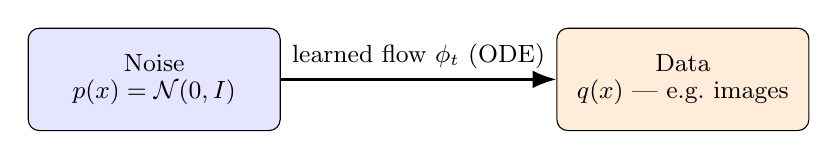
\begin{tikzpicture}[every node/.style={font=\small}]
\node[draw, rounded corners, fill=blue!10, minimum width=3.2cm, minimum height=1.3cm] (noise) {\shortstack{Noise\\$p(x) = \mathcal{N}(0,I)$}};
\node[draw, rounded corners, fill=orange!15, minimum width=3.2cm, minimum height=1.3cm, right=3.5cm of noise] (data) {\shortstack{Data\\$q(x)$ --- e.g.\ images}};
\draw[-{Latex[length=3mm]}, thick] (noise) -- node[above]{learned flow $\phi_t$ (ODE)} (data);
\end{tikzpicture}
\end{center}
\end{frame}
\begin{frame}{Continuous Normalizing Flows (CNFs)}
A \textbf{flow} is a time-dependent map $\phi_t:\mathbb{R}^d \to \mathbb{R}^d$ built from a \textbf{vector field} $v_t$ by solving an ODE:
\[
\frac{d}{dt}\phi_t(x) = v_t\big(\phi_t(x)\big), \qquad \phi_0(x) = x.
\]
Pushing samples from the prior through $\phi_t$ traces out a path of distributions:
\[
p_t = [\phi_t]_* \, p_0, \qquad p_0 = p_{\text{prior}}, \quad p_1 \approx p_{\text{data}}.
\]
\vspace{-4mm}
\begin{center}
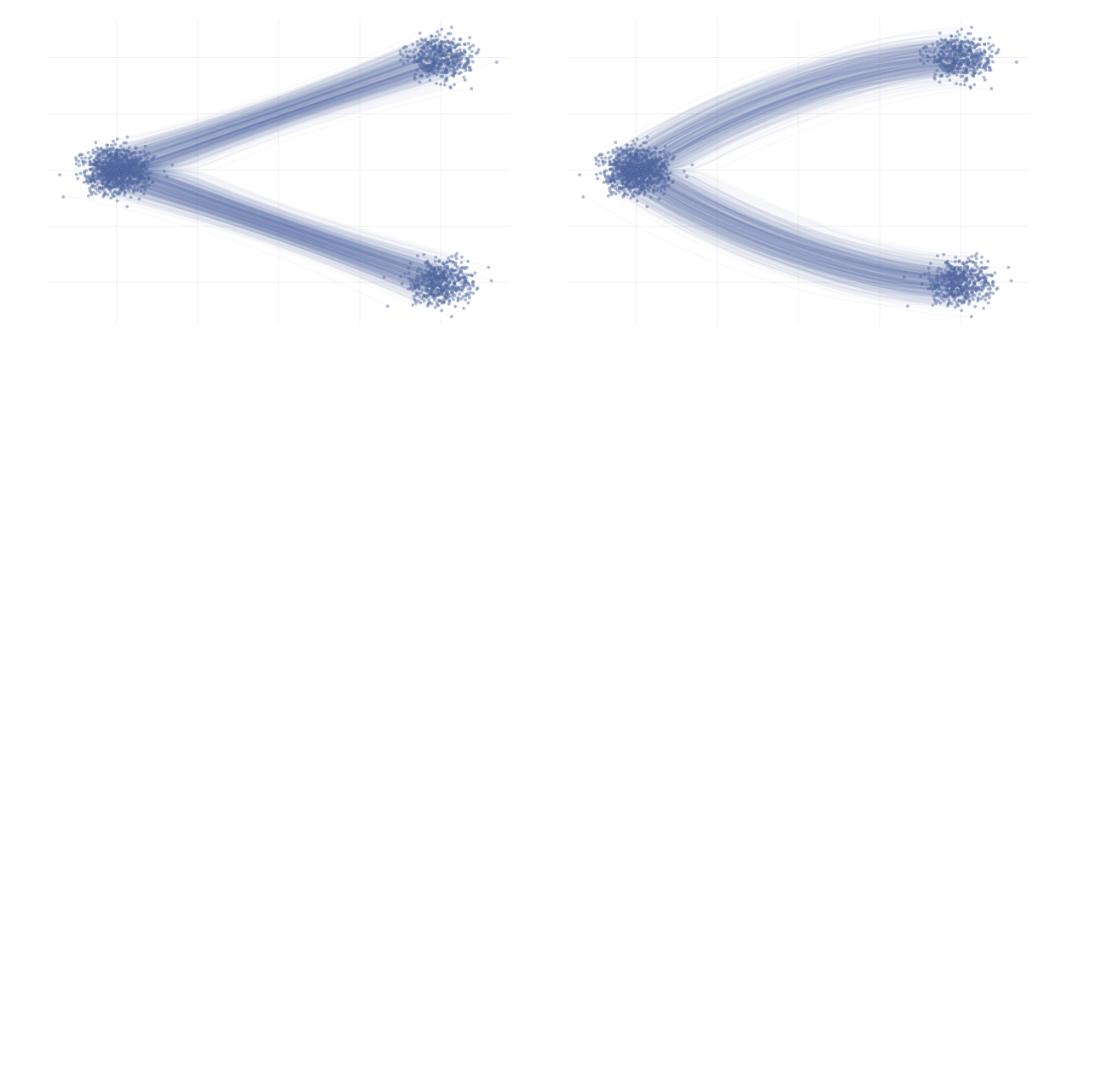
\includegraphics[width=0.2\textwidth]{fig7_nonunique_paths.png}
\end{center}
\vspace{-4mm}
{\tiny \textit{Many different vector fields can transport the same $p_{\text{prior}}$ into the same $p_{\text{data}}$ --- source: Fjelde, Mathieu \& Dutordoir (2024), Cambridge MLG blog.}}\\
\footnotesize \textbf{Intuition:} $v_t$ is a ``wind field'' that pushes every noise particle towards the data over $t\in[0,1]$.
\end{frame}
\begin{frame}{The Flow Matching objective}
If we knew a vector field $u_t$ that generates the correct marginal path $p_t$ (with $p_0 = p_{\text{prior}}$, $p_1 = q$), we could regress a network $v_t(x;\theta)$ onto it:
\[
\mathcal{L}_{FM}(\theta) = \mathbb{E}_{t \sim U[0,1],\, x \sim p_t(x)} \big\| v_t(x;\theta) - u_t(x) \big\|^2.
\]
\begin{itemize}
\item Problem: $p_t, u_t$ depend on the \emph{whole} dataset $q$ --- no closed form.
\item Solution: build them from simple \textbf{per-example} paths instead.
\end{itemize}
\end{frame}
\begin{frame}{Building the marginal path from conditional paths}
Each data point $x_1 \sim q$ gets its own simple \textbf{conditional path} $p_t(x|x_1)$ from $p_{\text{prior}}$ to $\delta_{x_1}$.
Averaging over all data points gives the \textbf{marginal path}:
\[
p_t(x) = \int p_t(x|x_1)\, q(x_1)\, dx_1.
\]
\vspace{-2mm}
\begin{center}
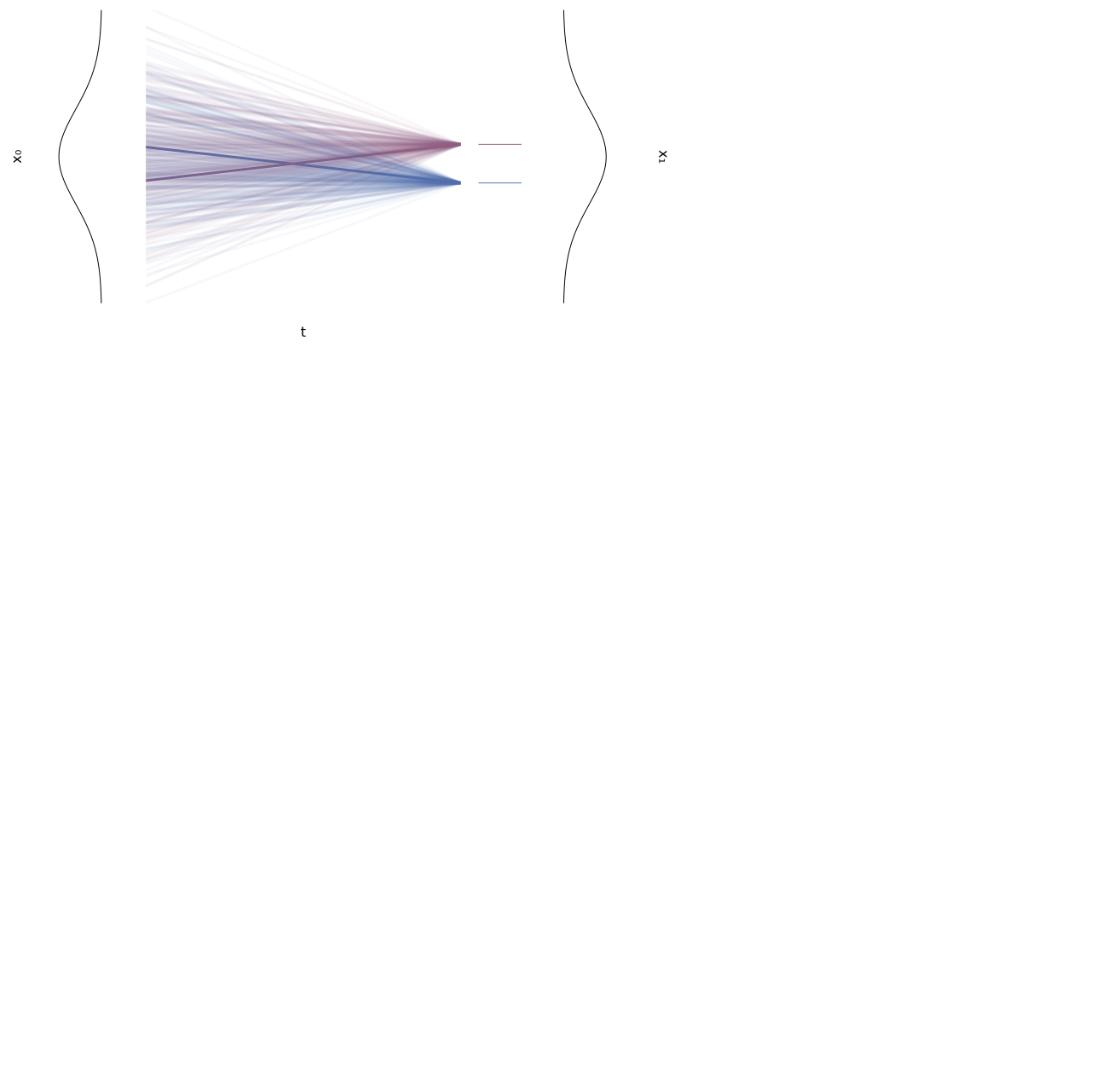
\includegraphics[width=0.33\textwidth]{fig8_conditional_flows.png}
\end{center}
\vspace{-2mm}
{\tiny \textit{Two conditional flows $\phi_t(x\mid x_1)$, one per data point --- source: Fjelde, Mathieu \& Dutordoir (2024), Cambridge MLG blog.}}\\[0.5mm]
{\footnotesize \textbf{Theorem (marginal vector field).} If $u_t(\cdot|x_1)$ generates $p_t(\cdot|x_1)$, then $u_t(x) = \int u_t(x|x_1)\, \frac{p_t(x|x_1) q(x_1)}{p_t(x)}\, dx_1$ generates $p_t$.}
\end{frame}

\begin{frame}{Conditional Flow Matching (tractable!)}
Instead of the intractable $\mathcal{L}_{FM}$, regress directly onto the simple conditional vector field:
\[
\mathcal{L}_{CFM}(\theta) = \mathbb{E}_{t,\, x_1 \sim q,\, x \sim p_t(x|x_1)} \big\| v_t(x;\theta) - u_t(x|x_1) \big\|^2.
\]
Every term is known: pick $x_1$, sample $x$ from its conditional path, regress $v_t$ onto $u_t(x|x_1)$.
\begin{center}
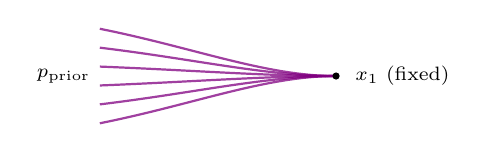
\begin{tikzpicture}[scale=0.6]
\foreach \y in {-1.0,-0.6,-0.2,0.2,0.6,1.0} {
\draw[violet, thick, opacity=0.75] (0,\y) .. controls (2,\y*0.6) and (3.5,0) .. (5,0);
}
\filldraw[black] (5,0) circle (1.8pt);
\node[left] at (0,0) {\scriptsize $p_{\text{prior}}$};
\node[right] at (5.2,0) {\scriptsize $x_1$ (fixed)};
\end{tikzpicture}
\end{center}\textbf{Key theorem:} $\mathcal{L}_{FM}$ and $\mathcal{L}_{CFM}$ have the \emph{same gradient} in $\theta$.
\end{frame}

\begin{frame}{Why do the gradients match? (proof sketch)}
Expand the squared norm and drop terms constant in $\theta$:
\[
\|v_t(x;\theta) - u_t(x)\|^2 \;\dot=\; \|v_t(x;\theta)\|^2 - 2\langle v_t(x;\theta), u_t(x)\rangle,
\]
where $\dot=$ means equal up to a $\theta$-independent constant. Using the definition of $u_t(x)$ as a conditional expectation:
\[
\mathbb{E}_{p_t(x)}\big[\langle v_t(x;\theta), u_t(x)\rangle\big]
= \mathbb{E}_{q(x_1)}\, \mathbb{E}_{p_t(x|x_1)}\big[\langle v_t(x;\theta), u_t(x|x_1)\rangle\big].
\]
This is Fubini's theorem plus $u_t(x) = \mathbb{E}_{q(x_1|x)}[u_t(x|x_1)]$, so $\mathcal{L}_{FM}(\theta) \dot= \mathcal{L}_{CFM}(\theta)$.
\end{frame}

\begin{frame}{A concrete choice: Gaussian conditional paths}
Let each conditional path be Gaussian:
\[
p_t(x|x_1) = \mathcal{N}\big(x \,\big|\, \mu_t(x_1),\, \sigma_t(x_1)^2 I\big),
\]
with $\mu_0=0,\sigma_0=1$ (prior) shrinking to $\mu_1=x_1,\sigma_1=\sigma_{\min}\approx 0$ (data point), generated by the linear map
\[
\psi_t(x) = \sigma_t(x_1)\, x + \mu_t(x_1), \qquad x \sim \mathcal{N}(0,I).
\]
\textbf{Theorem (closed-form conditional vector field).}
\[
u_t(x|x_1) = \frac{\sigma_t'(x_1)}{\sigma_t(x_1)}\big(x - \mu_t(x_1)\big) + \mu_t'(x_1).
\]
\begin{center}
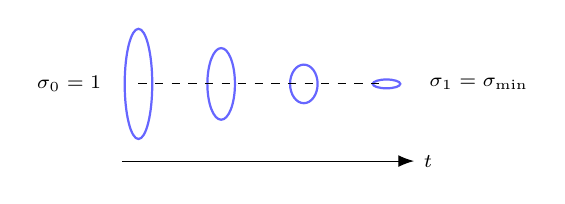
\begin{tikzpicture}[scale=0.7]
\draw[-{Latex[length=2mm]}] (-0.3,-1.4) -- (5,-1.4) node[right]{\scriptsize $t$};
\foreach \x/\w in {0/1.0, 1.5/0.65, 3/0.35, 4.5/0.08} {
\draw[blue!60, thick] (\x,0) ellipse (0.25 and \w);
}
\draw[dashed] (0,0) -- (4.5,0);
\node[left] at (-0.5,0) {\scriptsize $\sigma_0=1$};
\node[right] at (5.1,0) {\scriptsize $\sigma_1=\sigma_{\min}$};
\end{tikzpicture}
\end{center}
\end{frame}

\begin{frame}{Special case: the Optimal-Transport (straight-line) path}
Choosing $\mu_t(x_1) = t\,x_1$ and $\sigma_t(x_1) = 1-(1-\sigma_{\min})t$ gives straight-line conditional trajectories:
\[
\psi_t(x) = \big(1-(1-\sigma_{\min})t\big)\, x + t\, x_1, \qquad
u_t(x|x_1) = \frac{x_1 - (1-\sigma_{\min})\, x}{1-(1-\sigma_{\min})t}.
\]
Particles move along \textbf{straight lines} from noise to data at constant speed --- contrast with diffusion-style paths (e.g.\ VP/VE), whose trajectories are \textbf{curved}.
\begin{center}
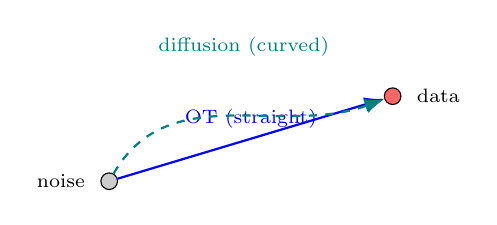
\begin{tikzpicture}[scale=0.9]
\node[draw, circle, fill=gray!40, minimum size=6pt, inner sep=0pt] (n) at (0,0) {};
\node[draw, circle, fill=red!60, minimum size=6pt, inner sep=0pt] (d) at (4,1.2) {};
\node[left=2pt of n] {\scriptsize noise};
\node[right=2pt of d] {\scriptsize data};
\draw<2->[-{Latex[length=2.5mm]}, thick, blue] (n) -- (d) node[midway, above] {\scriptsize OT (straight)};
\draw<3->[-{Latex[length=2.5mm]}, thick, teal, dashed] (n) to[out=60,in=200] (d);
\node<3->[teal] at (1.9,1.9) {\scriptsize diffusion (curved)};
\end{tikzpicture}
\end{center}
\end{frame}

\begin{frame}{Sampling: solving the ODE}
Once $v_t(x;\theta)$ is trained, generating new samples is simple integration:
\[
x_0 \sim p_{\text{prior}}, \qquad \frac{dx_t}{dt} = v_t(x_t;\theta), \qquad x_1 = \text{generated sample}.
\]
Simplest numerical solver --- \textbf{Euler's method} with step size $\Delta t = 1/N$:
\[
x_{t+\Delta t} = x_t + \Delta t \cdot v_t(x_t;\theta).
\]
\begin{itemize}
\item Repeat for $N$ steps from $t=0$ to $t=1$.
\item Fewer steps $\Rightarrow$ faster sampling but more discretization error --- this tension motivates later one-step methods (Mean Flow and friends) that we'll cover next.
\end{itemize}
\end{frame}

\begin{frame}{Recap: the Flow Matching recipe}
\begin{enumerate}
\item Pick a simple \textbf{conditional} probability path $p_t(x|x_1)$ per data point (e.g.\ Gaussian / OT straight line).
\item It has a known, closed-form conditional vector field $u_t(x|x_1)$.
\item Train a network $v_t(x;\theta)$ with the simple regression loss $\mathcal{L}_{CFM}$.
\item The gradient-equivalence theorem guarantees this also matches the true marginal vector field $u_t(x)$ generating $p_{\text{prior}} \to q$.
\item At sample time, integrate the ODE from noise at $t=0$ to data at $t=1$.
\end{enumerate}
\end{frame}


\section{Part 2 -- What is Mean Flow?}

\begin{frame}
\centering
{\Huge Part 2}\\[0.5em]
{\LARGE What is Mean Flow?}\\[1.5em]
\normalsize From many small steps to a single leap: one-step generative modeling\\[0.3em]
Based on Geng, Deng, Bai, Kolter \& He (2025) --- \textit{Mean Flows for One-step Generative Modeling}
\end{frame}

\begin{frame}{Recap: the cost of iterative sampling}
\begin{itemize}
\item Flow Matching learns the \textbf{instantaneous velocity} $v(z_t,t)$ --- the tangent direction of the flow at each instant.
\item Even with straight \emph{conditional} paths, the \emph{marginal} field is generally curved (Part 1).
\item Generating a sample means solving an ODE with many small Euler steps:
\[
z_{t+\Delta t} = z_t + \Delta t \, v(z_t,t).
\]
\end{itemize}
\begin{center}
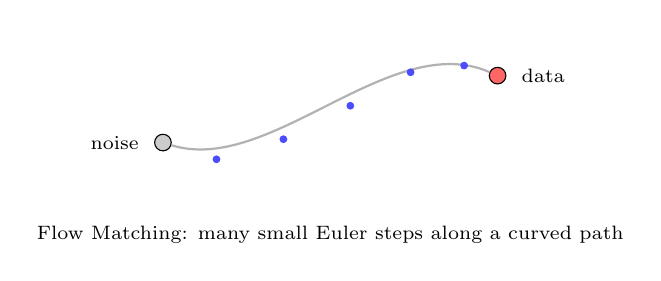
\begin{tikzpicture}[scale=0.85]
\node[draw, circle, fill=gray!40, minimum size=6pt, inner sep=0pt] (n) at (0,0) {};
\node[draw, circle, fill=red!60, minimum size=6pt, inner sep=0pt] (d) at (5,1) {};
\node[left=2pt of n] {\scriptsize noise};
\node[right=2pt of d] {\scriptsize data};
\draw[gray!60, thick] (n) .. controls (1.6,-0.5) and (3.4,1.7) .. (d);
\filldraw<2->[blue!70] (0.8,-0.25) circle (1.4pt);
\filldraw<3->[blue!70] (1.8,0.05) circle (1.4pt);
\filldraw<4->[blue!70] (2.8,0.55) circle (1.4pt);
\filldraw<5->[blue!70] (3.7,1.05) circle (1.4pt);
\filldraw<6->[blue!70] (4.5,1.15) circle (1.4pt);
\node<6->[below] at (2.5,-1.1) {\scriptsize Flow Matching: many small Euler steps along a curved path};
\end{tikzpicture}
\end{center}
\textbf{Question:} can we learn a field that lets us jump straight from noise to data in \emph{one} step?
\end{frame}

\begin{frame}{From instantaneous to average velocity}
Define the \textbf{average velocity} between two times $r<t$ as the displacement divided by the time interval:
\[
u(z_t,r,t) \;\triangleq\; \frac{1}{t-r}\int_r^t v(z_\tau,\tau)\, d\tau.
\]
\begin{itemize}
\item $v(z_t,t)$: instantaneous velocity --- tangent to the path.
\item $u(z_t,r,t)$: average velocity --- points along the \emph{displacement} $z_t-z_r$, generally \emph{not} aligned with $v$.
\end{itemize}
\begin{center}
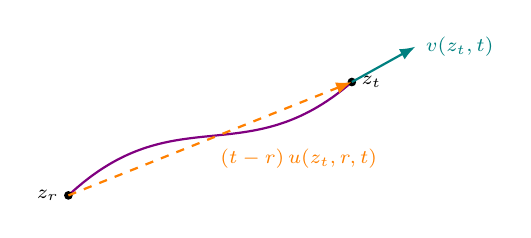
\begin{tikzpicture}[scale=0.9]
\draw[thick, violet] (0,0) .. controls (1.5,1.4) and (2.5,0.3) .. (4,1.6);
\filldraw[black] (0,0) circle (1.5pt) node[left]{\scriptsize $z_r$};
\filldraw[black] (4,1.6) circle (1.5pt) node[right]{\scriptsize $z_t$};
\draw<2->[-{Latex[length=2mm]}, thick, teal] (4,1.6) -- ++(0.9,0.5) node[right]{\scriptsize $v(z_t,t)$};
\draw<3->[-{Latex[length=2mm]}, thick, orange, dashed] (0,0) -- (4,1.6) node[midway, below right]{\scriptsize $(t-r)\,u(z_t,r,t)$};
\end{tikzpicture}
\end{center}
\end{frame}

\begin{frame}{Two natural properties of $u$}
\begin{itemize}
\item \textbf{Boundary case:} as $r\to t$, the interval shrinks to a point and
\[
\lim_{r\to t} u(z_t,r,t) = v(z_t,t).
\]
\item \textbf{Consistency:} one big jump over $[r,t]$ equals two smaller consecutive jumps over $[r,s]$ and $[s,t]$, for any $s$ in between:
\[
(t-r)\,u(z_t,r,t) = (s-r)\,u(z_s,r,s) + (t-s)\,u(z_t,s,t).
\]
This follows directly from additivity of the integral in the definition of $u$.
\end{itemize}
\begin{center}
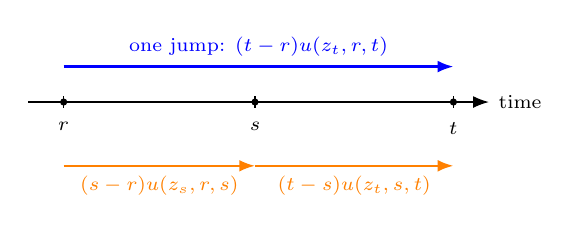
\begin{tikzpicture}[scale=0.9]
\draw[-{Latex[length=2mm]}] (0,0) -- (6.5,0) node[right]{\scriptsize time};
\foreach \x/\lab in {0.5/r, 3.2/s, 6/t}{
\draw (\x,0.08) -- (\x,-0.08);
\node[below] at (\x,-0.15) {\scriptsize $\lab$};
\filldraw[black] (\x,0) circle (1.2pt);
}
\draw<2->[-{Latex[length=2mm]}, thick, blue] (0.5,0.5) -- (6,0.5) node[midway, above]{\scriptsize one jump: $(t-r)u(z_t,r,t)$};
\draw<3->[-{Latex[length=2mm]}, thick, orange] (0.5,-0.9) -- (3.2,-0.9) node[midway, below]{\scriptsize $(s-r)u(z_s,r,s)$};
\draw<3->[-{Latex[length=2mm]}, thick, orange] (3.2,-0.9) -- (6,-0.9) node[midway, below]{\scriptsize $(t-s)u(z_t,s,t)$};
\end{tikzpicture}
\end{center}
\end{frame}

\begin{frame}{Deriving a trainable target: the MeanFlow Identity}
Rewrite the definition as $(t-r)\,u(z_t,r,t) = \int_r^t v(z_\tau,\tau)\,d\tau$, then differentiate both sides w.r.t.\ $t$ (holding $r$ fixed). Using the product rule on the left and the fundamental theorem of calculus on the right:
\[
u(z_t,r,t) + (t-r)\, \frac{d}{dt}u(z_t,r,t) = v(z_t,t).
\]
Rearranging gives the \textbf{MeanFlow Identity}:
\[
\underbrace{u(z_t,r,t)}_{\text{average vel.}} \;=\; \underbrace{v(z_t,t)}_{\text{instant. vel.}} \;-\; (t-r)\underbrace{\frac{d}{dt}u(z_t,r,t)}_{\text{time derivative}}.
\]
\textbf{Key idea:} this expresses $u$ purely in terms of quantities available during training --- no integral needed!
\end{frame}

\begin{frame}{Training with a Jacobian-vector product (JVP)}
The total derivative expands via the chain rule (with $\frac{dz_t}{dt}=v$, $\frac{dr}{dt}=0$, $\frac{dt}{dt}=1$):
\[
\frac{d}{dt}u(z_t,r,t) = v(z_t,t)\,\partial_z u + \partial_t u,
\]
a Jacobian-vector product computable in one extra backward pass (\texttt{jvp} in PyTorch/JAX). We train a network $u_\theta$ to match the identity, with a stop-gradient on the target:
\[
\mathcal{L}(\theta) = \mathbb{E}\, \big\| u_\theta(z_t,r,t) - \text{sg}(u_{\text{tgt}}) \big\|^2, \qquad
u_{\text{tgt}} = v_t - (t-r)\big(v_t\,\partial_z u_\theta + \partial_t u_\theta\big).
\]
\vspace{-4mm}
\begin{center}
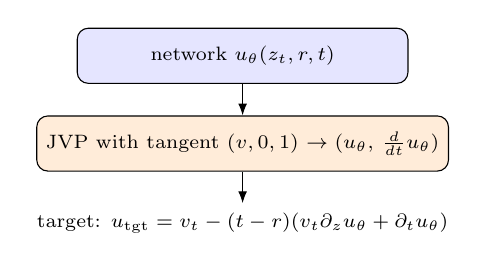
\begin{tikzpicture}[node distance=4mm, every node/.style={font=\scriptsize}]
\node[draw, rounded corners, fill=blue!10, minimum width=4.2cm, minimum height=0.7cm] (net) {network $u_\theta(z_t,r,t)$};
\node[draw, rounded corners, fill=orange!15, minimum width=4.2cm, minimum height=0.7cm, below=of net] (jvp) {JVP with tangent $(v,0,1)$ $\to (u_\theta,\, \tfrac{d}{dt}u_\theta)$};
\node[below=of jvp] (target) {\scriptsize target: $u_{\text{tgt}} = v_t - (t-r)(v_t\partial_z u_\theta + \partial_t u_\theta)$};
\draw[-{Latex[length=1.5mm]}] (net) -- (jvp);
\draw[-{Latex[length=1.5mm]}] (jvp) -- (target);
\end{tikzpicture}
\end{center}
\end{frame}

\begin{frame}{Sampling: one function evaluation}
Once trained, replace the ODE integral directly with the average velocity:
\[
z_r = z_t - (t-r)\, u_\theta(z_t,r,t).
\]
Setting $t=1,\, r=0$ gives \textbf{one-step generation}:
\[
z_0 = z_1 - u_\theta(z_1, 0, 1), \qquad z_1 = \epsilon \sim p_{\text{prior}}.
\]
\begin{center}
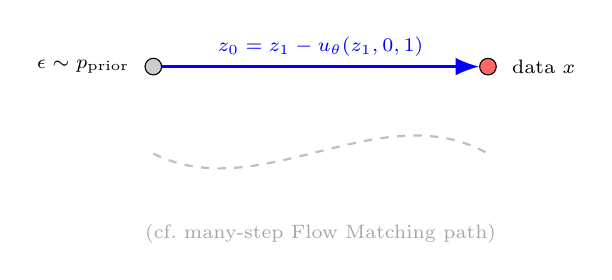
\begin{tikzpicture}[scale=0.85]
\node[draw, circle, fill=gray!40, minimum size=6pt, inner sep=0pt] (n) at (0,1) {};
\node[draw, circle, fill=red!60, minimum size=6pt, inner sep=0pt] (d) at (5,1) {};
\node[left=2pt of n] {\scriptsize $\epsilon\sim p_{\text{prior}}$};
\node[right=2pt of d] {\scriptsize data $x$};
\draw<2->[-{Latex[length=3mm]}, thick, blue] (n) -- (d) node[midway, above]{\scriptsize $z_0 = z_1 - u_\theta(z_1,0,1)$};
\draw<3->[gray!50, thick, dashed] (0,-0.3) .. controls (1.6,-1.1) and (3.4,0.6) .. (5,-0.3);
\node<3->[gray!70, below] at (2.5,-1.2) {\scriptsize (cf.\ many-step Flow Matching path)};
\end{tikzpicture}
\end{center}
\textbf{Note:} setting $r=t$ everywhere recovers ordinary Flow Matching --- MeanFlow strictly generalizes it.
\end{frame}

\begin{frame}{Recap: the Mean Flow recipe}
\begin{enumerate}
\item Define average velocity $u(z_t,r,t)$ as displacement over an interval, contrasting instantaneous velocity $v$.
\item Differentiate the definition to obtain the \textbf{MeanFlow Identity} relating $u$, $v$, and $\frac{d}{dt}u$.
\item Train a network $u_\theta$ by regressing onto this identity, computing $\frac{d}{dt}u_\theta$ with a single JVP.
\item Sample in \textbf{one step}: $z_0 = z_1 - u_\theta(z_1,0,1)$.
\end{enumerate}
\end{frame}


\section{Part 3 -- Improved Mean Flow}

\begin{frame}
\centering
{\Huge Part 3}\\[0.5em]
{\LARGE Improved Mean Flow}\\[1.5em]
\normalsize Fixing two hidden issues in the original recipe\\[0.3em]
Based on Geng, Lu, Wu, Shechtman, Kolter \& He (2025) --- \textit{Improved Mean Flows: On the Challenges of Fastforward Generative Models}
\end{frame}

\begin{frame}{A crack in the original recipe}
\begin{itemize}
\item MeanFlow works remarkably well, but a closer look reveals a subtle issue.
\item \textbf{A self-referential target.} The training target for $u_\theta$ is built using $u_\theta$ itself (via the JVP). This is not a standard regression problem: the target moves as the network changes.
\end{itemize}
\begin{center}
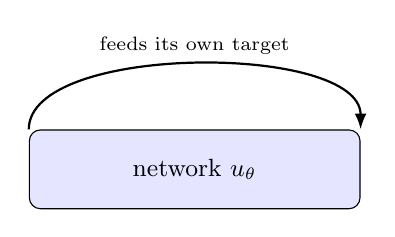
\begin{tikzpicture}[node distance=10mm, every node/.style={font=\small}]
\node[draw, rounded corners, fill=blue!10, minimum width=4.2cm, minimum height=1cm] (net) {network $u_\theta$};
\draw[-{Latex[length=2mm]}, thick] (net.north west) .. controls +(0,1.1) and +(0,1.1) .. (net.north east) node[midway, above]{\scriptsize feeds its own target};
\end{tikzpicture}
\end{center}
\end{frame}

\begin{frame}{Rewriting MeanFlow as a $v$-loss}
\small
Recall the MeanFlow identity, now solved for the instantaneous velocity:
\[
v(z_t) = u(z_t) + (t-r)\,\frac{d}{dt}u(z_t).
\]
\begin{itemize}
\item Original MF regresses $u_\theta$ onto a $u$-shaped target built from $u_\theta$ itself.
\item Flip the identity around: treat the \textbf{left-hand side} $v$ as an ordinary regression target, and the \textbf{right-hand side} as a compound function of $u_\theta$, call it $V_\theta$.
\item This gives a Flow-Matching-style loss: $\mathbb{E}\,\|V_\theta - (\epsilon - x)\|^2$.
\end{itemize}
\vspace{-3mm}
\begin{center}
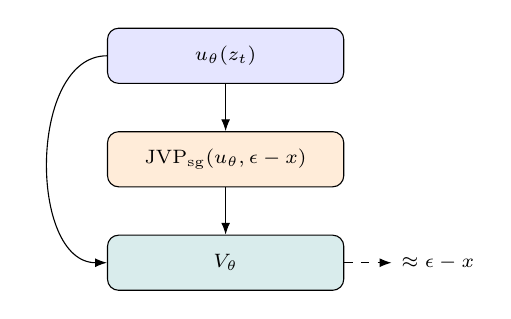
\begin{tikzpicture}[node distance=6mm, every node/.style={font=\scriptsize}]
\node[draw, rounded corners, fill=blue!10, minimum width=3.0cm, minimum height=0.7cm] (u) {$u_\theta(z_t)$};
\node[draw, rounded corners, fill=orange!15, minimum width=3.0cm, minimum height=0.7cm, below=of u] (jvp) {JVP$_{\text{sg}}(u_\theta,\epsilon-x)$};
\node[draw, rounded corners, fill=teal!15, minimum width=3.0cm, minimum height=0.7cm, below=of jvp] (V) {$V_\theta$};
\node[right=6mm of V] (target) {\scriptsize $\approx \epsilon - x$};
\draw[-{Latex[length=1.5mm]}] (u) -- (jvp);
\draw[-{Latex[length=1.5mm]}] (jvp) -- (V);
\draw[-{Latex[length=1.5mm]}] (u.west) .. controls +(-1.0,0) and +(-1.0,0) .. (V.west);
\draw[-{Latex[length=1.5mm]}, dashed] (V) -- (target);
\end{tikzpicture}
\end{center}
\end{frame}

\begin{frame}{The real fix: which vector feeds the JVP?}
\footnotesize
The $v$-loss rewrite (previous slide) is only algebra --- same stop-gradient, same loss value, same gradient. The one real difference is which direction $v$ is plugged into the JVP:
\[
\tfrac{d}{dt}u(z_t) \;=\; \partial_z u_\theta(z_t)\, v \;+\; \partial_t u_\theta(z_t)
\]
\begin{columns}[T]
\begin{column}{0.48\textwidth}
\centering
\scriptsize \textbf{Original MF: $v=\epsilon-x$}
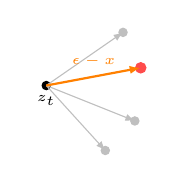
\begin{tikzpicture}[scale=0.75, every node/.style={font=\tiny}]
\filldraw[black] (0,0) circle (2pt) node[below]{$z_t$};
\filldraw[gray!50] (1.3,0.9) circle (2pt);
\filldraw[gray!50] (1.5,-0.6) circle (2pt);
\filldraw[gray!50] (1.0,-1.1) circle (2pt);
\filldraw[red!70] (1.6,0.3) circle (2.5pt);
\draw[gray!50, -{Latex[length=1.2mm]}] (0,0) -- (1.3,0.9);
\draw[gray!50, -{Latex[length=1.2mm]}] (0,0) -- (1.5,-0.6);
\draw[gray!50, -{Latex[length=1.2mm]}] (0,0) -- (1.0,-1.1);
\draw[orange, thick, -{Latex[length=1.4mm]}] (0,0) -- (1.6,0.3) node[midway, above]{\tiny $\epsilon-x$};
\end{tikzpicture}\\[1mm]
\scriptsize crossing paths $\Rightarrow$ arbitrary, high-variance direction
\end{column}
\begin{column}{0.48\textwidth}
\centering
\scriptsize \textbf{Improved MF: $v=v_\theta(z_t)$}
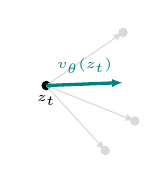
\begin{tikzpicture}[scale=0.75, every node/.style={font=\tiny}]
\filldraw[black] (0,0) circle (2pt) node[below]{$z_t$};
\filldraw[gray!30] (1.3,0.9) circle (2pt);
\filldraw[gray!30] (1.5,-0.6) circle (2pt);
\filldraw[gray!30] (1.0,-1.1) circle (2pt);
\draw[gray!30, -{Latex[length=1.2mm]}] (0,0) -- (1.3,0.9);
\draw[gray!30, -{Latex[length=1.2mm]}] (0,0) -- (1.5,-0.6);
\draw[gray!30, -{Latex[length=1.2mm]}] (0,0) -- (1.0,-1.1);
\draw[teal, very thick, -{Latex[length=1.4mm]}] (0,0) -- (1.3,0.05) node[midway, above]{\tiny $v_\theta(z_t)$};
\end{tikzpicture}\\[1mm]
\scriptsize aligned with the flow $\Rightarrow$ smooth, low-variance direction
\end{column}
\end{columns}
\vspace{1mm}
{\scriptsize Empirically (iMF paper, Fig.~3): with the same rewritten loss, the conditional-direction version trains noisy and non-decreasing, while the marginal-direction version drops smoothly.}
\end{frame}

\begin{frame}{A hidden issue: an illegitimate input}
\begin{itemize}
\item Our compound function is really $V_\theta(z_t,\, \epsilon - x)$ --- it secretly needs the \emph{conditional} velocity $\epsilon - x$, not just the noisy sample $z_t$.
\item That is not a legitimate prediction function, and the extra input injects high variance into the JVP term (training becomes noisy).
\item Fix: replace $\epsilon - x$ inside the JVP with the network's \textbf{own estimate} of the marginal velocity, $v_\theta(z_t)$.
\end{itemize}
\begin{center}
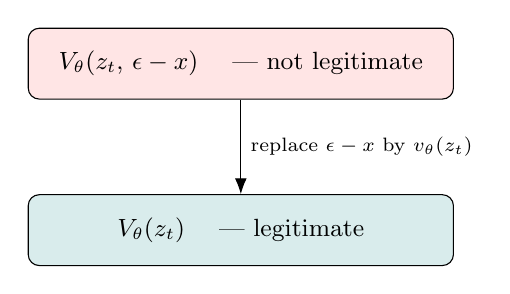
\begin{tikzpicture}[node distance=10mm, every node/.style={font=\small}]
\node[draw, rounded corners, fill=red!10, minimum width=5.4cm, minimum height=0.9cm] (a) {$V_\theta(z_t,\, \epsilon-x)$ \quad --- not legitimate};
\node[draw, rounded corners, fill=teal!15, minimum width=5.4cm, minimum height=0.9cm, below=12mm of a] (b) {$V_\theta(z_t)$ \quad --- legitimate};
\draw[-{Latex[length=2mm]}] (a) -- (b) node[midway, right]{\scriptsize replace $\epsilon-x$ by $v_\theta(z_t)$};
\end{tikzpicture}
\end{center}
\end{frame}

\begin{frame}{Fix: give the network its own $v$-estimate}
\begin{itemize}
\item \textbf{Boundary condition (free lunch).} By definition $v(z_t,t) \equiv u(z_t,t,t)$ --- average velocity over a zero-length interval \emph{is} the instantaneous velocity. So simply set $v_\theta(z_t,t) \triangleq u_\theta(z_t,t,t)$. No extra parameters.
\item \textbf{Auxiliary $v$-head.} Alternatively, branch a small extra head off the last few layers of $u_\theta$, trained with its own Flow-Matching loss. A few extra training-time parameters, none at inference.
\end{itemize}
\begin{center}
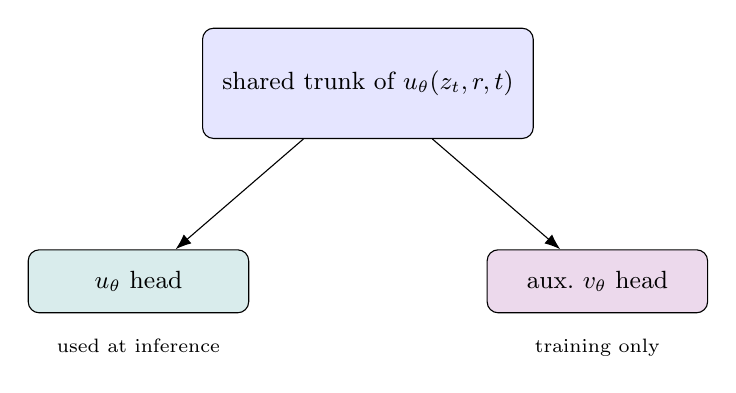
\begin{tikzpicture}[node distance=10mm, every node/.style={font=\small}]
\node[draw, rounded corners, fill=blue!10, minimum width=4.2cm, minimum height=1.4cm] (trunk) {shared trunk of $u_\theta(z_t,r,t)$};
\node[draw, rounded corners, fill=teal!15, minimum width=2.8cm, minimum height=0.8cm, below left=14mm and -6mm of trunk] (uhead) {$u_\theta$ head};
\node[draw, rounded corners, fill=violet!15, minimum width=2.8cm, minimum height=0.8cm, below right=14mm and -6mm of trunk] (vhead) {aux.\ $v_\theta$ head};
\draw[-{Latex[length=2mm]}] (trunk) -- (uhead);
\draw[-{Latex[length=2mm]}] (trunk) -- (vhead);
\node[below=2mm of uhead] {\scriptsize used at inference};
\node[below=2mm of vhead] {\scriptsize training only};
\end{tikzpicture}
\end{center}
\end{frame}

\begin{frame}{Recap: two fixes behind Improved Mean Flow}
\begin{enumerate}
\item \textbf{Legitimate regression target:} rewrite the MeanFlow identity as a $v$-loss, and feed the JVP its tangent from the network's own $v_\theta(z_t)$ estimate --- not from $\epsilon-x$.
\end{enumerate}
\vspace{0.5em}
Together, these turn MeanFlow from a promising recipe into a genuinely competitive one-step generator --- without any distillation from a pretrained teacher.
\end{frame}

\end{document}
